\section{Questão 12-9}

Nesta questão, analisamos a função da posição \(s(t)\) e determinamos a expressão para a velocidade \(v(t)\) em diferentes intervalos de tempo. Além disso, apresentamos os resultados em forma gráfica.

\subsection*{Função da Posição \(s(t)\)}
A função da posição \(s(t)\) é definida por:
\[
s(t) = 
\begin{cases} 
0.5t^2 & \text{se } t \leq 6, \\
108 & \text{se } t > 6.
\end{cases}
\]

\subsection*{Cálculo da Velocidade \(v(t)\)}
A velocidade \(v(t)\) é obtida pela derivada da posição \(s(t)\) em relação ao tempo \(t\). Para \(t \leq 6\), temos:
\[
s(t) = 0.5t^2 \implies v(t) = \frac{d}{dt}s(t) = t.
\]

Para \(t > 6\), como \(s(t)\) é constante (\(s(t) = 108\)), a velocidade é:
\[
v(t) = 0.
\]

Portanto, a velocidade \(v(t)\) é definida por:
\[
v(t) = 
\begin{cases} 
t & \text{se } t \leq 6, \\
0 & \text{se } t > 6.
\end{cases}
\]

\subsection*{Dados Gerados}
Os dados de tempo (\(t\)), posição (\(s(t)\)), e velocidade (\(v(t)\)) foram gerados e organizados para análise. A tabela a seguir ilustra os valores calculados (valores exemplares):

\begin{table}[H]
    \centering
    \begin{tabular}{|c|c|c|}
        \hline
        \textbf{Tempo (s)} & \textbf{Posição (m)} & \textbf{Velocidade (m/s)} \\
        \hline
        0.0 & 0.0 & 0.0 \\
        1.0 & 0.5 & 1.0 \\
        2.0 & 2.0 & 2.0 \\
        \vdots & \vdots & \vdots \\
        6.0 & 18.0 & 6.0 \\
        7.0 & 108.0 & 0.0 \\
        8.0 & 108.0 & 0.0 \\
        \hline
    \end{tabular}
    \caption{Dados de posição e velocidade em função do tempo.}
\end{table}

\subsection*{Gráfico de Velocidade \(v(t)\)}
A função \(v(t)\) foi representada graficamente. O eixo \(x\) corresponde ao tempo (\(t\)), enquanto o eixo \(y\) corresponde à velocidade (\(v(t)\)). Uma linha vertical foi traçada em \(t = 6\), indicando a mudança no comportamento da função.

\begin{figure}[H]
    \centering
    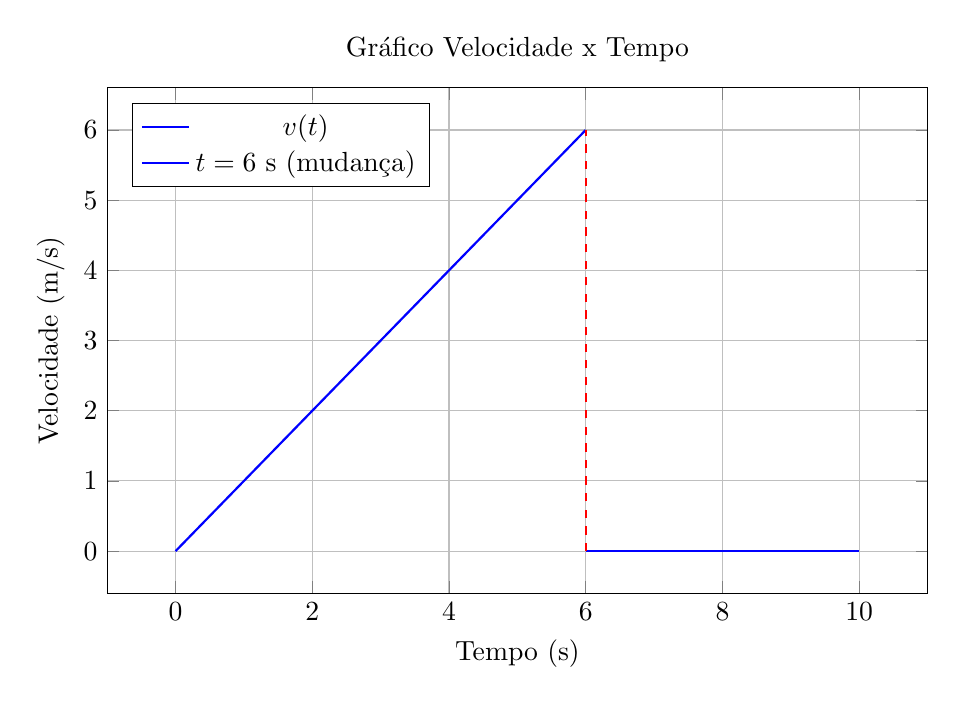
\begin{tikzpicture}
    \begin{axis}[
        width=12cm, height=8cm,
        xlabel={Tempo (s)},
        ylabel={Velocidade (m/s)},
        grid=major,
        legend pos=north west,
        title={Gráfico Velocidade x Tempo}
    ]
        \addplot[domain=0:6, samples=100, blue, thick] {x};
        \addplot[domain=6:10, samples=100, blue, thick] {0};
        \addplot[dashed, red, thick] coordinates {(6, 0) (6, 6)};
        \legend{$v(t)$, $t = 6$ s (mudança)};
    \end{axis}
    \end{tikzpicture}
    \caption{Gráfico da função velocidade \(v(t)\).}\label{fig:figure}
\end{figure}

\subsection*{Resultados Finais}
\begin{itemize}
    \item Função da posição:
    \[
    s(t) = 
    \begin{cases} 
    0.5t^2 & \text{se } t \leq 6, \\
    108 & \text{se } t > 6.
    \end{cases}
    \]
    \item Função da velocidade:
    \[
    v(t) = 
    \begin{cases} 
    t & \text{se } t \leq 6, \\
    0 & \text{se } t > 6.
    \end{cases}
    \]
\end{itemize}
